% \begin{tikzpicture}[text centered]
	\draw[legende] (-3.25,2.5) rectangle (11.25,-4);
	\node at (4,2.1) {\strong{création de séquences dégradées par partie avec des dégradations synthétiques}};
	\node at (0,0) {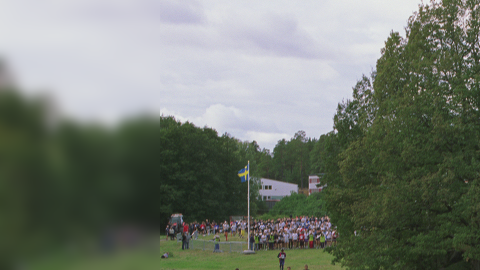
\includegraphics[width=6cm]{img/chap3/aboveMarathonFlou}};
	\draw (-1,1.7) -- (-1,-1.7);
	\node at (-2,1.2) {flou};
	\node at (4,0) {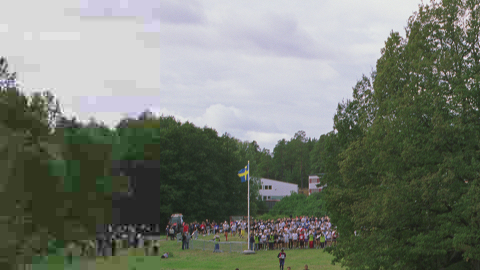
\includegraphics[width=6cm]{img/chap3/aboveMarathonBloc}};
	\draw (3,1.7) -- (3,-1.7);
	\node at (2,1.2) {effet de bloc};
	\node at (8,0) {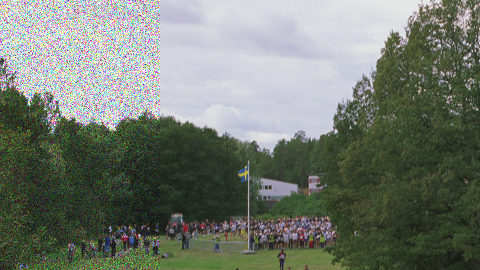
\includegraphics[width=6cm]{img/chap3/aboveMarathonBruit}};
	\draw (7,1.7) -- (7,-1.7);
	\node at (6,1.2) {bruit};
	\node at (2.5,-2) {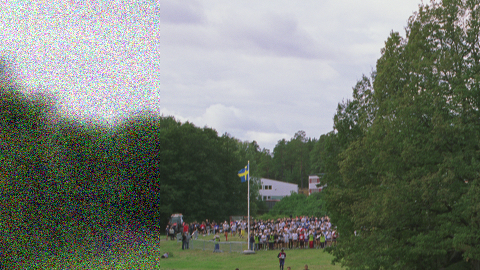
\includegraphics[width=6cm]{img/chap3/aboveMarathonFlouBruit.png}};
	\draw (1.5,-0.3) -- (1.5,-3.7);
	\node at (0.5,-0.8) {bruit+flou};
	\node at (5.5,-2) {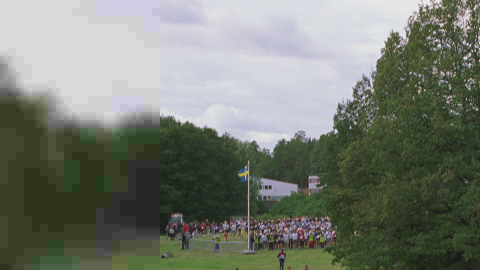
\includegraphics[width=6cm]{img/chap3/aboveMarathonBlocFlou.png}};
	\draw (4.5,-0.3) -- (4.5,-3.7);
	\node[text width=1.5cm] at (3.5,-0.8) {effet de bloc+flou};
	\node at (9,-2) {\dots};

	\node[action,text width=6cm] (node) at (0,-5.5) {tests de détection, description, mesure de gêne et d'intensité};
	\draw[fleche] (0,-4) -- (node);
	\draw[fleche] (node) -- (4,-5.5);

	\foreach \x in {4,4.5,5,5.5}
	{
			\draw[legende] (\x,-6.25) rectangle (\x + 1.5,-4.5);
			\draw[->] (\x + .25,-5.75) -- (\x + 1.25,-5.75);
			\draw[->] (\x + .25,-5.75) -- (\x + .25,-4.75) node[above=-0.1cm, font=\tiny] {gêne};
	}
	\node[below, font=\tiny] at (6.75,-5.75) {$I_{\mathit{flou}}$};
	\node[text width=5cm] at (5.5,-7) {une fonction de gêne par combinaison de dégradations};
	\draw[fleche] (7,-5.5) -- (8,-5.5);

	\draw[->] (8.5,-6.5) -- (10.5,-6.5) node[below] {$f(I_{\mathit{flou}}, \dots)$};
	\draw[->] (8.5,-6.5) -- (8.5,-4.5) node[right] {gêne};
% \end{tikzpicture}
